\chapter{Internet of Things}

The main topics addressed aside from \textbf{IoT} itself are how it relates to \textit{Machine Learning} and \textit{Cloud} computing processes, but also \textit{IoT interoperability}, known \textit{Standards}, and the \textit{security} concerns about IoT.

\section{IoT introduction}
\textbf{Cyber and Physical Systems} (CPS) operate in both the Physical and Cyber worlds, thus we can see IoT as an embodiement of CPSs.

In a \textit{smart environment}, smart objects are both physical and cyber, hence they are subject to ``physical experiences'' such as being placed, moved, damaged and so on.
\begin{center}
   But actually\dots\\
   \ul{What is a \textit{smart environment}?}
\end{center}

The answer actually ain't trivial;
a journal on IoT reports:
\begin{center}
\textit{``smart environments can be defined with a variety of different characteristics based on the applications they serve, their interaction models with humans, the practical system design aspects, as well as the multi-faceted conceptual and algorithmic considerations that would enable them to operate seamlessly and unobtrusively''}
\end{center}

\section{Platforms for IoT}
Sensors and actuators are the edge of the cloud.
In general the purpose of IoT is to gather and send data, send it somewhere where it gets transformed into information ultimately used to provide some functionality for an end user, or it simply presented to them.

A \textbf{Platform for IoT} is essentially a ---complex--- software hosted on the cloud, which, first of all, \ul{\textbf{collects} data gathered by IoT devices, but \textit{not} only that}:
\begin{itemize}
   \item Identification
   \item Discovery
   \item Device Management
   \item Abstraction/virtualization
   \item Service composition\\
   Integrating services of different IoT devices and SW components into a composite service
   \item Semantics
   \item Data Flow management
   \begin{itemize}
      \item $sensors \longrightarrow applications$
      \item $applications \ra sensors$
      \item Support for aggregation, processing, analytics
   \end{itemize}
\end{itemize}

\section{No-SQL Databases}
\textbf{No-SQL} DBs address the problem of the several changes of data formats, sources, cardinality and so on, which happen throughout time.

A common example is \textbf{MongoDB}, which stores records in JSON-like objects called \textit{documents}, which are stored in \textit{collections}, the entity corresponding to tables in relational DBs,
with the key difference that multiple documents in a single collection may be structured differently.

\section{IoT Issues}
\begin{paracol}{2}
   
   \begin{itemize}
      \item Performance
   \item Energy Efficiency
   \item Security
   \item Data analysis/processing
   \begin{itemize}
      \item Adaptability/personalization
   \end{itemize}
   \note{The course will cover the basics of signal processing, with mentions to machine learning}
\end{itemize}
\switchcolumn

\begin{itemize}
   \item Communication/brokerage/binding
   \item Data representation
   \item Interoperability
   \note{
      Standard discussed will be ZigBee, MQTT, and IEEE 802.15.4 (?)
      }
   \end{itemize}
\end{paracol}

\begin{figure}[htbp]
   \centering
   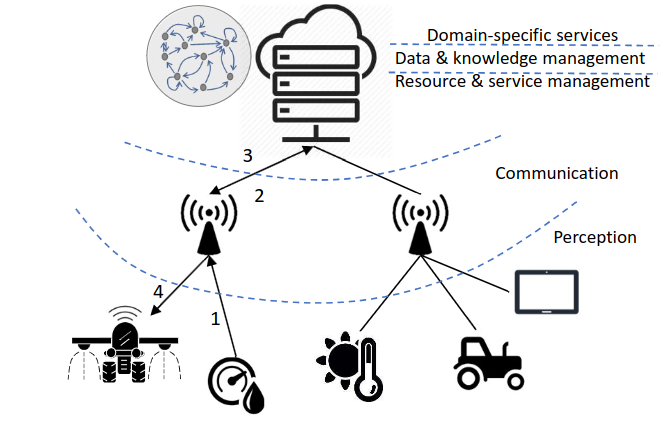
\includegraphics{images/iot_communication.png}
   \caption{Communication outline in IoT}
   IoT systems are distributed, and servers may be dislocated around the globe, making room for \ul{\textbf{latency} and \textbf{reliability} issues}.
   \label{fig:iot_communication}
\end{figure}

To confine the problem displayed in Fig. \ref{fig:iot_communication} there are proposal to move the ability to make a decision on the data closer to the edge, but this in general isn't trivial.

\labelitemize{\textit{\ul{Key Issues}}}{
   \begin{enumerate}
      \item Producing and handling fast-streaming heterogeneous sensed data
      \item Make devices context-aware \& allow them for continuous adaptation
      \item Handle strong computing and energy constraints
   \end{enumerate}
   }

\subsection{Edge and Fog computing}
   \begin{figure}[htbp]
      \centering
      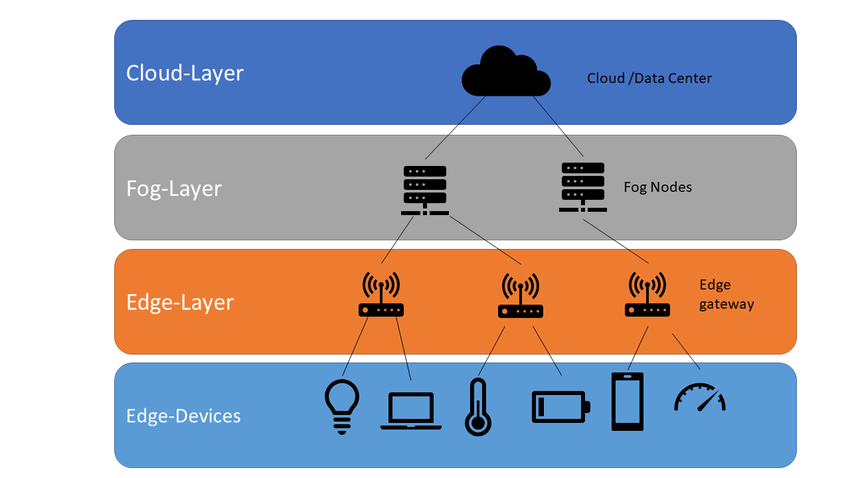
\includegraphics{images/fogedge.png}
      \caption{Layers scheme}
      \label{fig:fogedge}
   \end{figure}
A solution forsees to split the network in 4 layers, allowing for different response times and decisional capabilities.

A gateway on the \textbf{edge} interconnects the IoT-enabled devices with the higher-level communication networks, performing protocol translations.

A basic task performed at the fog layer is  aggregating and collecting data, and then flushing it to the cloud periodically.

However, some decisions on the aggregated data may be taken at the fog node without querying the cloud, for instance determining where is a nest of tortoises, whether an explosion has occurred (by analyzing data from multiple sensors), and ---maybe, one day in a not-so-far future--- recognize human language.
\note{prof. Chessa developed an 8 bit controller implementing a model for determining where is a nest of tortoises.\\
\textit{Alexa} and \textit{Google Home} currently send audio samples to the cloud for processing, but in the futurue this may be done locally.}


\subsection{Artificial Intelligence}
AI splits into \textbf{Machine Learning} and \textbf{Curated Knowledge}.
\note{\textit{ML} focuses on mimicking how humans \ul{\textit{learn}} on new knowledge, while \textit{curated knowledge} focuses on mimicking how humans \ul{\textit{reason}} on a known set of data.}

Machine Learning reveals itself to be particularly useful in aggregatin multiple heterogeneous time-series sensed data about the same environment.
\note{Supervised and Reinforcement learning are more promising than}


\subsection{Blockchain \& IoT}
A \textbf{blockchain} may act as a shared ledger between companies in a supply chain, with IoT devices to track goods and to monitor their quality along the chain, i.e. production stages, shipping and distribution.\\
With a blockchain each actor along the supply chain can \ul{query the ledger to check the ---certified--- state of the goods}.

\subsection{Interoperability}
\labelitemize{\textit{Vertical Silos}}{
\begin{adjustwidth}{1em}{0em}
Developing a straight implementation of an IoT solution, starting from physical up to the application layer, is not a problem by itself.\\
In this way solution you implemented will work only on your devices, making your intervention needed for any change or update;
besides, products by other vendors will be incompatible. 
\end{adjustwidth}
}

\textit{Vertical Silos} business model leads to \textbf{vendor lock-in}s, which basically are service limitations which prevent the users from purchasing and using products from other vendors.
\nl
\nl

The solution to avoid ---or limit--- such issues is to introduce \ul{\textbf{standards}}.
Standards require common interests and agreements among different manufacturers, they are usually motivated by a reductino of the costs for development of a technology.
There must be ``\textit{coopetition}" among manufacturers.
\note{
   There is coopetition usually when a \ul{technology becomes \textbf{mature}}:
   \ns
\begin{itemize}[topsep=0pt,partopsep=0em]
   \item Big revenues are somewhere else
   \item No interest in investing big money in developing the technology
   \item[$\Rightarrow$] Without these conditions the standards will most likely fall
\end{itemize}} 

\note{For what concerns wireless communication, standards are mainly differentiated by \textit{Range} and \textit{Data Rate}.
}

However, interoperability may be an issue not strictly related to vertical silos, but also to standards, in case there are \textit{too many}.\\
The problem of interoperability shifts from low-level to application level.\\
To solve the problem, \textbf{gateways} are introduced, which translate different protocols.

\newpage
\begin{figure}[htbp]
   \centering
   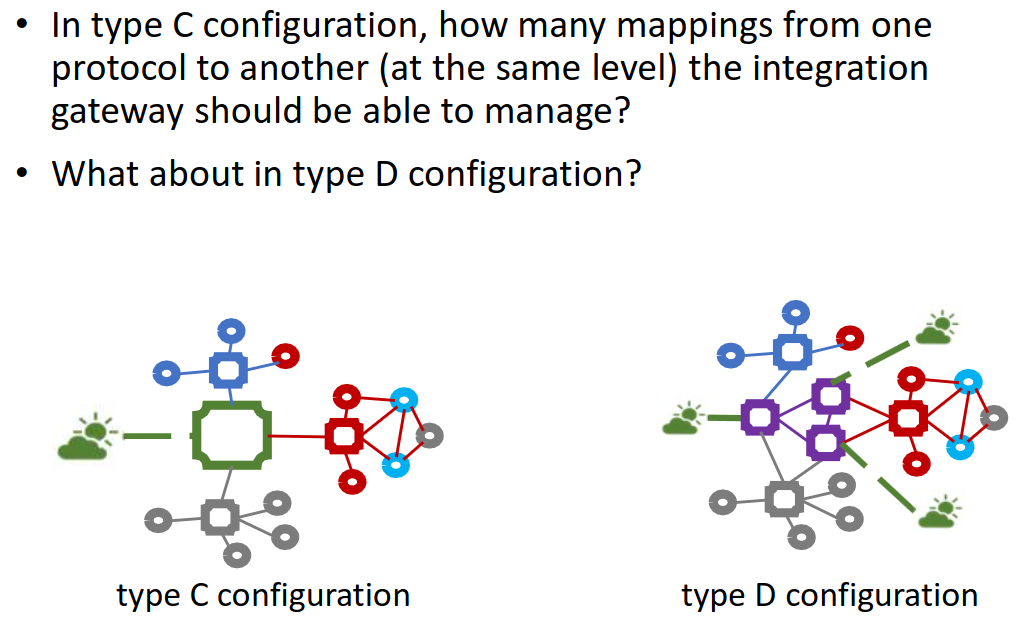
\includegraphics{images/gateways_configs.png}
   \caption{Gateway configs}
   \label{fig:gateways_configs}
\end{figure}
Considering Fig \ref{fig:gateways_configs} and assuming $n$ protocol standards, the gateway in config C must be able to manage a mapping for every possible pair of standards,
resulting in $n*n = n^2$ mappings.
In configuration D instead evey gateway translates \textit{from} and \textit{to} an \textbf{intermediate language} ({\color{mauve}purple} in figure), resulting in a double translation process, but only $2*n$ mappings, which is much less.



\section{Security in IoT}
\begin{figure}[htbp]
   \centering
   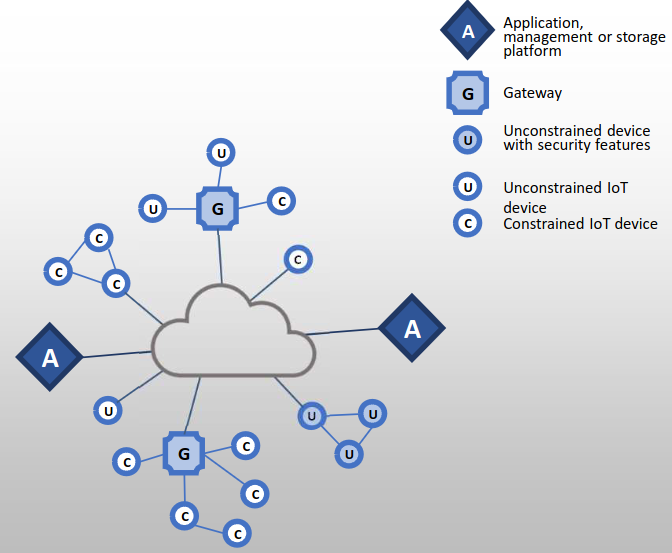
\includegraphics{images/securityelements.png}
   \caption{Security elements of interest}
   \label{fig:securityelements}
\end{figure}
In an IoT environment there are various elements, each with its characteristics and vulnerabilities.

In general there are many issues concerning \textbf{patching vulnerabilities}, which poorly ---or not at all--- addressed.
\begin{itemize}
   \item There is a crisis point with regard to the security of embedded
   systems, including IoT devices
   \item 
   The embedded devices are riddled with vulnerabilities and there is no
   good way to patch them
   \item Chip manufacturers have strong incentives to produce their product as quickly and cheaply as possible
   \item The device manufacturers focus is the functionality of the device itself
   \item The end user may have no means of patching the system or, if so, little information about when and how to patch
   \item The result is that the hundreds of millions of Internet-connected
   devices in the IoT are vulnerable to attacks
   \item This is certainly a problem with sensors, allowing attackers to insert false data into the network
   \note{Not so critical for wristbands, but potentially harmful for water quality sensors, even worse for uranium enrichment, or aircraft sensors}
   \item It is potentially a graver threat with actuators, where the attacker can affect the operation of machinery and other devices
\end{itemize}

\note{What about \textbf{confidentiality}? Is it necessary?\\
The lecturer provided an example:\\
Assume that a wristband records the heartbeat without enforcing confidentiality, and assume that such heartbeat indicates a risk of heart disease in the owner.
The owner may want to have a life insurance, but if a company had bought the unconfidential data on the black market, and recognized that the owner may suffer from a heart disease.
Then the company could rise the price of the insurance for the unconfidential wristband owner.
}

Aside from these, laws introduce many requirements concerning security, which may be critical to satisfy in an IoT environment.
In particular, The \texttt{IUT-T} standard Recommendation \texttt{Y.2066} includes a list of security requirements for the IoT, which concern the following points, but note that the document \ul{does \textbf{not} define how to enforce and satisfy such requirements}:
\ns
\begin{itemize}
   \item Communication security
   \item Data management security
   \item Service provision security
   \item Integration of security policies and techniques
   \item Mutual authentication and authorization\\
   It it crucial for the authentication to work both directions, from the gateway to the device, and from the device to the gateway.
   It is needed because wireless networks are easily trickable by intruders. 
   \item Security audit
\end{itemize}
\nl

\begin{paracol}{2}
   Considering the points mentioned above, we must consider what is the role of \textbf{gateways} about security.

   Sometimes instead of mutual one, weaker \textit{one-way authentication} may be enforced:
   either the device authenticates itself to the gateway or
   the gateway authenticates itself to the device,
   but not both.
   
   Also the security of the data is not trivial to achieve, especially if constrained devices are used, because they may not be able to enforce task such as encryption or authentication.
   
   This makes \textbf{privacy} concers arise especially regarding homes, cars and retail outlets, because with massive IoT, governments and private enterprises
   are able to collect massive amounts of data about individuals.
   \switchcolumn

   \begin{figure}[htbp]
      \centering
      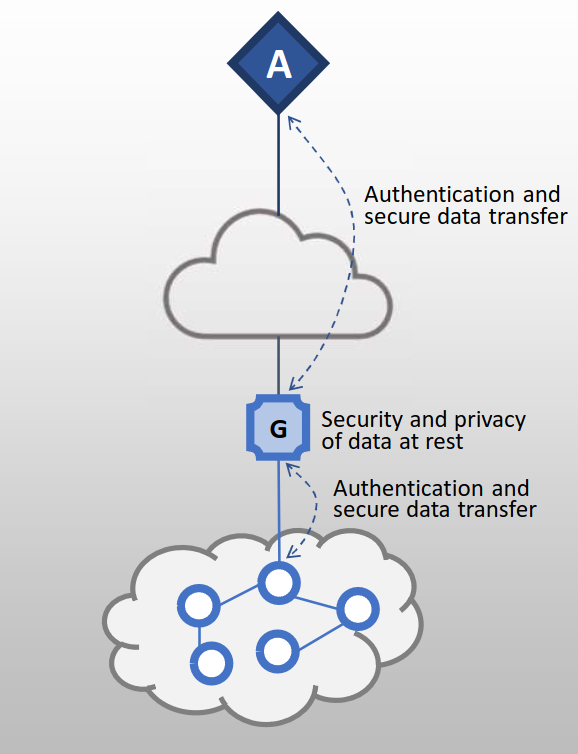
\includegraphics{images/gateways_security.png}
      \caption{Gateways security functions}
      \label{fig:gateways_security}
   \end{figure}
\end{paracol}
